\documentclass[border=4pt]{standalone}

\usepackage{amsmath}
\usepackage{tikz}
\usepackage{mathdots}
\usepackage{yhmath}
\usepackage{cancel}
\usepackage{color}
\usepackage{siunitx}
\usepackage{array}
\usepackage{multirow}
\usepackage{amssymb}
\usepackage{gensymb}
\usepackage{tabularx}
\usepackage{booktabs}
\usetikzlibrary{fadings}
\usetikzlibrary{patterns}


\begin{document}
 


\tikzset{every picture/.style={line width=0.75pt}} %set default line width to 0.75pt        

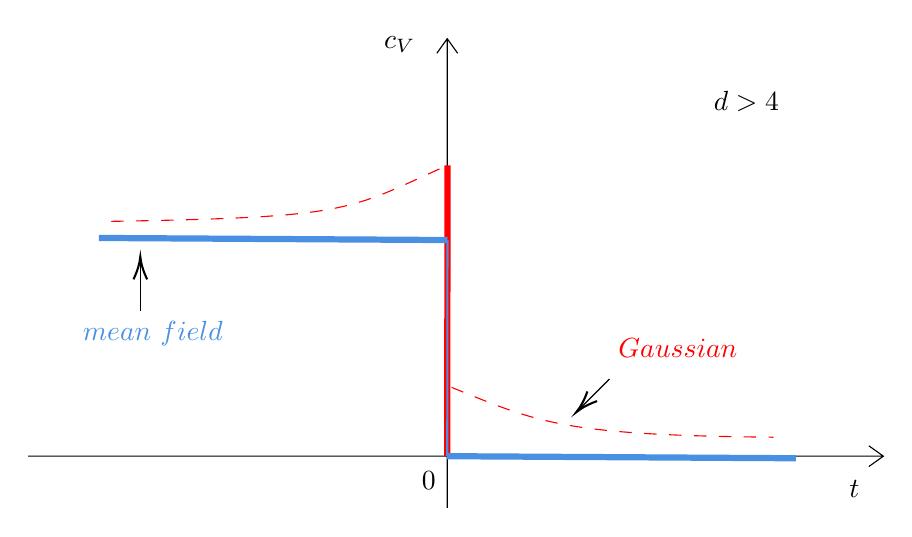
\begin{tikzpicture}[x=0.75pt,y=0.75pt,yscale=-1,xscale=1]
%uncomment if require: \path (0,300); %set diagram left start at 0, and has height of 300

%Shape: Axis 2D [id:dp15475147511122245] 
\draw  (78,223.14) -- (490,223.14)(279.88,22) -- (279.88,248) (483,218.14) -- (490,223.14) -- (483,228.14) (274.88,29) -- (279.88,22) -- (284.88,29)  ;
%Straight Lines [id:da1712333151889378] 
\draw [color={rgb, 255:red, 255; green, 0; blue, 0 }  ,draw opacity=1 ][line width=2.25]    (280,83) -- (279.88,223.14) ;


%Straight Lines [id:da3952399338041339] 
\draw [color={rgb, 255:red, 74; green, 144; blue, 226 }  ,draw opacity=1 ][line width=2.25]    (112,118) -- (280,119) ;


%Straight Lines [id:da30186176524476793] 
\draw [color={rgb, 255:red, 74; green, 144; blue, 226 }  ,draw opacity=1 ][line width=2.25]    (279.88,223.14) -- (447.88,224.14) ;


%Straight Lines [id:da5438451239749351] 
\draw [color={rgb, 255:red, 74; green, 144; blue, 226 }  ,draw opacity=1 ][line width=0.75]    (280,119) -- (279.88,223.14) ;


%Curve Lines [id:da4415690563976402] 
\draw [color={rgb, 255:red, 255; green, 0; blue, 0 }  ,draw opacity=1 ] [dash pattern={on 4.5pt off 4.5pt}]  (118,110) .. controls (234,108) and (231,105) .. (280,83) ;


%Curve Lines [id:da6156587721788513] 
\draw [color={rgb, 255:red, 255; green, 0; blue, 0 }  ,draw opacity=1 ] [dash pattern={on 4.5pt off 4.5pt}]  (282,190) .. controls (324,207) and (335,213) .. (437,214) ;


%Straight Lines [id:da023237301719628567] 
\draw    (132,153) -- (132,129) ;
\draw [shift={(132,127)}, rotate = 450] [color={rgb, 255:red, 0; green, 0; blue, 0 }  ][line width=0.75]    (10.93,-3.29) .. controls (6.95,-1.4) and (3.31,-0.3) .. (0,0) .. controls (3.31,0.3) and (6.95,1.4) .. (10.93,3.29)   ;

%Straight Lines [id:da4144228695644414] 
\draw    (358,186) -- (343.41,200.59) ;
\draw [shift={(342,202)}, rotate = 315] [color={rgb, 255:red, 0; green, 0; blue, 0 }  ][line width=0.75]    (10.93,-3.29) .. controls (6.95,-1.4) and (3.31,-0.3) .. (0,0) .. controls (3.31,0.3) and (6.95,1.4) .. (10.93,3.29)   ;


% Text Node
\draw (271,235) node    {$0$};
% Text Node
\draw (476,239) node    {$t$};
% Text Node
\draw (257,25) node    {$c_{V}$};
% Text Node
\draw (138,164) node  [color={rgb, 255:red, 74; green, 144; blue, 226 }  ,opacity=1 ]  {$mean\ field$};
% Text Node
\draw (391,171) node  [color={rgb, 255:red, 255; green, 0; blue, 0 }  ,opacity=1 ]  {$Gaussian$};
% Text Node
\draw (424,52) node    {$d >4$};


\end{tikzpicture}
\end{document}
